\chapter{Introduction to Algorithmic Design}

\section{Computation and Computerisation}

Today, in almost all engineering and architectural fields, computers are used heavily and almost exclusively for any type of work. Some of the utilisation of computers in architecture such as 3D NURBS or Mesh modelling programs, or any mouse manipulated 3D forms programmes, are often thought to be computational. Although they essentially use numerical computation to display or `translate' \cite{terzidis06} different forms, ultimately it is the user who willingly manipulates the models.  This is a confusion between computation and computerisation. 

\paragraph{Computerisation}could be defined as using the computer as a tool instead of traditional tools or media. One could use ink and paper to write a letter, or use a word processor instead. The presentation is probably better, the work is done faster, but the content would not change on account of this tool swap. The same notion basically applies to CAD programmes, which are merely tools to draw shapes in a manner which essentially replaces pencil and paper; in both cases the user is in complete control of the outcome.

\paragraph{Computation}on the other hand produces that which was not entirely planned out by the user, it creates unpredicted results. The input in this case is not the final product. This input constraints the process towards a roughly imagined product; but does not completely define it. This is due to the fact that computation is used in areas where humans are very limited; such as calculation and processing of large numbers. The same applies to architectural modelling; one could use computation to enter a formula that would render a cube, but that is never the case. Computation is utilised in producing objects of high complexity, or in large numbers with a wide spectrum of variation that would make it impossible for the user to manually model.

To reiterate the above stated; the product of computation --- even though the algorithms that govern it and the input it needs are a product of the human mind --- is not solely a product of the human mind, but a product of a parallel logic.

\section{Parallel Logic}

Algorithms solve problems in a finite number of steps; either deterministically, or stochastically\footnote{Stochastic: Involving a random variable \cite{merriam03}}. The problems it solves can be a specific problem or an exploration of the unknown. The logic it uses, was designed by people, which might imply that algorithm is a subset of human logic. The fact is: it is not.

The way computers rationalise is different from how people think; it is in fact inconceivable by humans, the same way a human's rationalisation is virtually impossible for a computer to emulate.  This is due to the fact that computers can process enormous amounts of abstract data and numbers, such as the `Brute force' technique which processes `all' possibilities of a solution, which could be thousands or millions of solutions. On the other hand, it cannot perceive `intuition', personal preference; things that are unique to a human's mind and require emotion,subconscious reactions.

\paragraph{Algorithms,}or procedures, are a description of steps to accomplish a specific task, which ``\emph{allow abstraction and encapsulation of complexity and re-usability}''\cite{hernandez06}. In abstraction; procedures have three parts:
\begin{enumerate}
  \item The name of the procedure, which is the handle by which the procedure is called.
  \item The arguments, which are the parameters used within the procedure. These are similar to ingredients in a recipe.
  \item The description of the procedure, which is the recipe itself. Within this process the user inputs values into parameters\footnote{Parameters are a series of arguments which take up values in a function, and are also the placeholder of variable value.}, the procedure makes calculations according to the description of the procedures and outputs the result to the user. The calculation part is usually hidden from the user, which is called encapsulation.
\end{enumerate}

\section{Geometric Modelling and Design as Algorithms}

The question is whether a paradigm of logic such as algorithms is capable of producing architectural design. This can be answered by starting at the fact that architectural design is ultimately composed of interrelated geometrical objects.

The way geometry is defined is very specific to the different types of geometry being defined. A point is defined by three variables of space, a line is defined by two points each holding three values in space\ldots etc, with the addition of more complex modelling techniques such as Boolean operations. This nature of geometrical definitions requires specific procedures, each having a different set of encapsulated parameters. Therefore, geometric modelling is a parametric procedure. \cite{hernandez06}

\begin{figure}[htbp]
\flushleft
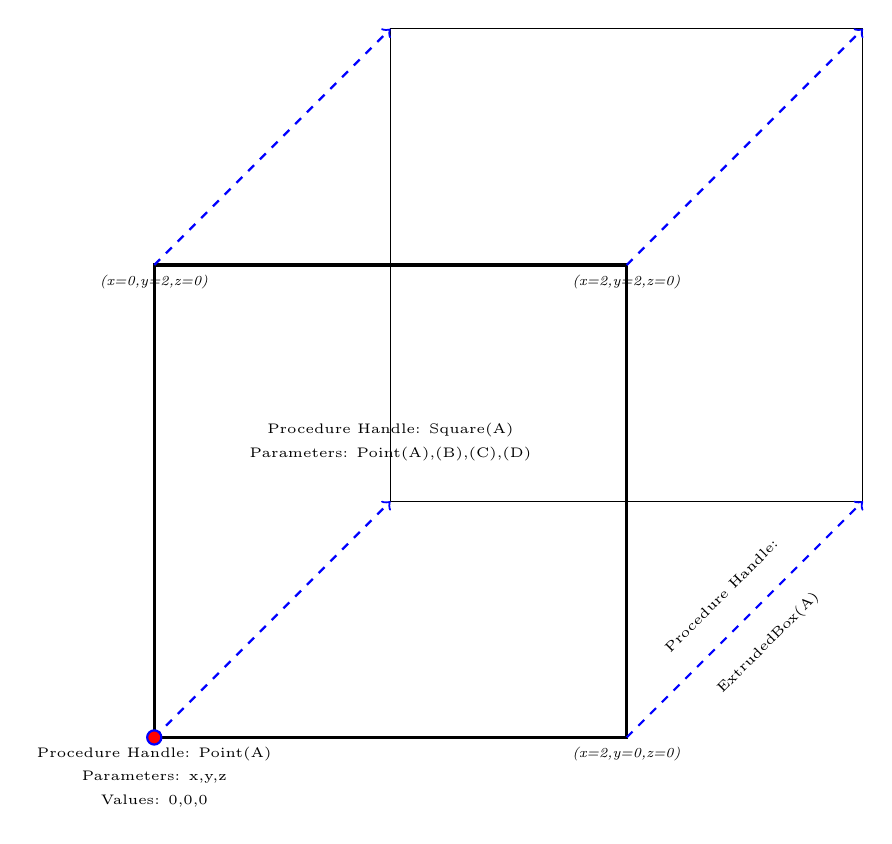
\begin{tikzpicture}[scale=3]
\draw [very thick] (0,0) --(0,2) --(2,2) --(2,0) --(0,0);
\draw (1,1) --(1,3) --(3,3) --(3,1) --(1,1);
\draw [->,dashed,thick,blue] (0,0) --(1,1);
\draw [->,dashed,thick,blue] (0,2) --(1,3);
\draw [->,dashed,thick,blue] (2,2) --(3,3);
\draw [->,dashed,thick,blue] (2,0) --(3,1);
\draw [thick,blue,fill=red](0,0) circle [radius=0.03];
\node [below] at (0,0) {\tiny Procedure Handle: Point(A)};
\node [below] at (0,-0.1) {\tiny Parameters: x,y,z};
\node [below] at (0,-0.2) {\tiny Values: 0,0,0};
\node [below] at (0,2) {\tiny \emph{(x=0,y=2,z=0)}};
\node [below] at (2,2) {\tiny \emph{(x=2,y=2,z=0)}};
\node [below] at (2,0) {\tiny \emph{(x=2,y=0,z=0)}};
\node at (1,1.3) {\tiny Procedure Handle: Square(A)};
\node at (1,1.2) {\tiny Parameters: Point(A),(B),(C),(D)};
\node at (2.4,0.6) [rotate=45] {\tiny Procedure Handle:};
\node at (2.6,0.4) [rotate=45] {\tiny ExtrudedBox(A)};
\end{tikzpicture}
\centering
\vspace{5mm}
\caption[Procedures and Parameters in Algorithmic Modelling]{Procedures and Parameters in Algorithmic Modelling. {\footnotesize Point procedure with three parameters, a square procedure with points as parameters, and a cube extrusion procedure with the square as a parameter}}
\label{SqrAnalysis}
\end{figure}

In some cases, design can be also be defined by procedures, when it is possible to break down into a step-by-step repetitive process, which also contain arguments (Parameters) that alter the design with variable values.

When design is treated as a procedure; with parameters defining different designs with different values; numbers, relations, shapes and operations are also treated as parameters. A cube for example can be defined by extruding a square along it's perpendicular axe, which makes the square in this case a parameter of the extrusion procedure (Figure \ref{SqrAnalysis}).

Algorithmic design can be summarised as: ``\emph{A procedure carrying instructions in a systematic order where all geometrical components that represent a design are parameterised}''\cite{hernandez06}. Algorithmic design can also be defined as \emph{rule-based} design; consisting of a solid set of consequetive instructions that govern an action to produce a desired outcome, while noting that in this particular case; the outcome does not necessarily match the intent. \label{AlgoGeoModel}
